% archived by dlw Jan 2018 (written circa Aug 2017)
%\documentclass[a4paper]{article}
\documentclass[11pt]{article}
\usepackage{graphicx}
\usepackage{amsfonts}
\usepackage{amsmath}
\usepackage{algorithm}
\usepackage{algpseudocode}
\usepackage{multirow}
%\usepackage{minted}

\makeatletter
\def\BState{\State\hskip-\ALG@thistlm}
\makeatother

\graphicspath{ {images/} }
\setlength{\parindent}{0.0in}
\setlength{\parskip}{0.1in}
\setlength{\textheight}{8.5in}
\setlength{\textwidth}{5.9in} %.7
\setlength{\topmargin}{-.48in}
\setlength{\oddsidemargin}{.1in} %.29
\renewcommand{\thebibliography}[1]{\vspace{2\baselineskip}\noindent
           {\large\bf Bibliography}\small
           \nopagebreak\vspace{.5\baselineskip}\nopagebreak
           \list{[\arabic{enumi}]}{\settowidth{\labelwidth}{[#1]}
           \leftmargin\labelwidth \advance\leftmargin\labelsep
           \usecounter{enumi}}
           \def\newblock{\hskip .11em plus .33em minus -.07em}
           \sloppy \sfcode`\.=1000\relax}
% fixes heading for bibliography
\newcommand{\Vector}[1]{#1}  %{\mbox{{\boldmath $#1$}}}
\newcommand{\Matrix}[1]{#1}   %{\mbox{{\boldmath $#1$}}}
\newcommand{\VectLen}[1]{\mid\Vector{#1}\mid}
\newcommand{\Rint}[1]{\int_{#1}^{\infty}}
%\newcommand{\Size}[1]{\| #1 \|}
\newcommand{\Size}[1]{\mid #1 \mid}
\newcommand{\Floor}[1]{\lfloor #1 \rfloor}
\newcommand{\Ceil}[1]{\left\lceil #1 \right\rceil}
\def\Argmin{\mathop{\rm argmin}}
\renewcommand{\baselinestretch}{1}


%% Language and font encodings
\usepackage[english]{babel}
%\usepackage[utf8x]{inputenc}
%\usepackage[T1]{fontenc}

%% Sets page size and margins
\usepackage[a4paper,top=3cm,bottom=2cm,left=3cm,right=3cm,marginparwidth=1.75cm]{geometry}

%% Useful packages
\usepackage{amsmath}
\usepackage{graphicx}
\usepackage[colorinlistoftodos]{todonotes}
\usepackage[colorlinks=true, allcolors=blue]{hyperref}

\title{ARCHIVED \\Simulator Analysis and Prometheus comparison}
\author{Jaime Carrasco, Cristobal Pais}

\begin{document}
\maketitle

\begin{abstract}
SimName is a new cells-based fire spread simulator. It includes a wide range of options that gives flexibility to the user when performing simulations such as statistical analysis, graphical outputs, GIS interaction, etc. In addition, a parallel implementation for high performance computers is included, allowing the users to take advantage of this approach when performing large-scale simulations. Its outputs are already integrated with optimization software like AMPL or PYOMO. It has been completely programmed in Python.
\end{abstract}

\section{Introduction}

In order to evaluate methods for creating forest harvest plans in the presence of forest fires, fire spread must
be simulated.
We will begin with some assumptions:
\begin{enumerate}
	\item Harvest plans are issued and then executed each year. \label{list:planfreq}
	\item Harvesting takes place before fires.
	\item Replanting is soon after harvest. \label{list:replant}
	\item Hourly time resolution is sufficient for modeling the spread of fire. \label{list:stepsize}
	\item Harvest planning is done for {\em harvest blocks} and fire spread is modeled using {\em fire cells} that are much smaller.
\end{enumerate}

Any of these assumptions could be relaxed later. Since the time
resolution is the most pervasive and most likely to be changed, we
will eschew the use of ``hour'' and ``hourly'' and instead refer to
{\em time steps} with the understanding that we mean ``fire simulation time
steps'' and in initial experiments, we mean simply ``hours'' but we
won't use that word.


Assumption~\ref{list:planfreq} implies that the basic time
step for computing values and costs is one year. \\
Assumption~\ref{list:replant} is relevant for simulations that run for a large number of years.\\
Assumption~\ref{list:stepsize} is strong, fire can be modeled within minutes, good as a first approach.


\textbf{Simulator scheme}\\
In order to represent the problem's dynamic, figure \ref{tline} shows the different events in the forest. At the beginning of every year we have a \textit{HPeriod }(Harvest Period) where we take harvest decisions - before fire dynamics - and every stand/block is replanted soon after these actions. After this \textit{HPeriod}, \textit{FPeriods }(Fire Periods) start, where all the ignitions and fire spread happen. Important is to note that for the moment we are working without a particular time step size, avoiding confusions about the length of each period.

\begin{figure}[h!]
\centering
\includegraphics[scale=0.9]{TimeLine.png}
\caption{\label{tline} Scheme of fire simulator.}	 
\end{figure}

Fire will start at some point - remembering that there is a specific fire season during summer - and then the fire spread model will start to simulate the fire dynamics using the weather and other information inside the simulator (probability of an ignition or fire spread). In figure \ref{Periods}, as an example we can see a forest with 9 stands/blocks where a fire ignites in the first \textit{FPeriod }- after the first \textit{HPeriod }- in cell 4 and then it spreads to different harvest units for two more \textit{FPeriods }(note that the harvest decision was to not touch the forest, since all the forest's cells are available). After these periods, a new \textit{HPeriod }(next year) starts. 

\begin{figure}[h!]
	\centering
	\includegraphics[scale=0.8]{Periods.png}
	\caption{\label{Periods} Simulation example}
\end{figure}
Where:
\begin{itemize}
	\item $H_{t_{h}} = $ Harvest plan for $HPeriod$ $t_{h}$
	\item $R_{t_{h}} = $ Reforestation plan during $HPeriod $ $t_{h}$
	\item $FI_{i,t_{f}} = 1 $ if fire ignites in cell/block $i$ during $ FPeriod $ $t_{f}$
	\item $FS_{j,i,t_{f}} = 1 $ if fire spreads from cell/block $j$ to cell/block $i$ during $ FPeriod $ $t_{f}$
\end{itemize}

\textbf{Note}: \textit{HPeriods }and \textit{FPeriods }do not need to be in the same time scale, we just need them to be consistent. See appendix for details and examples for this idea, applied in a stochastic multi-stage model, including an explanation of \textit{FI} and \textit{FS}.

Then, we can define two main time sets: Harvest Periods (\textit{HPeriods}) indicating the beginning of each year (independent of the time step size) and Fire Dynamic periods (\textit{FPeriods}) where ignitions and fire spreads occur. Important is to note - again - that these sets can use different time scales if they are consistent.\\

\newpage
We can define them in a general way:
\begin{itemize}
	\item Set \textit{Periods }:= $\lbrace \textit{t} \in \mathbb{Z^{+}} \rbrace $
	\item Set \textit{HPeriods }:= $ \lbrace t_{h} \in Periods: t_{h} = 1 + \alpha(1+h)$  where $\alpha \in \mathbb{Z}^{+}_{0}, h$ is the fire period size$\rbrace$
	\item Set \textit{FPeriods }:= $\lbrace t_{f} \in \bigcup_{t_{h}=1} [t_{h}+1,t_{h}+h] \rbrace $
\end{itemize}

\textbf{Example:}
Using 40 periods as the total planning horizon, h = 9 hours and harvesting after every fire period we have:
\begin{itemize}
	\item Set \textit{Periods }:= $\lbrace 1,...,40\rbrace $
	\item Set \textit{HPeriods }:= $ \lbrace 1,1+1*10=11,1+2*10=21,31\rbrace$
	\item Set \textit{FPeriods }:= $[2,10] \bigcup [12,20] \bigcup [22,30] \bigcup [32,40] $
\end{itemize}

 



\section{SimName: Stochastic Cell-based simulator}
SimName is a stochastic fire ignition \& spread cell-based simulator developed in Python. It allows the user to simulate the fire dynamics inside a grid instance that can represent a real forest based on variables such as weather, fuel type of each cell, elevation (terrain components), ignition points, spotting probability, etc. \\

Its flexibility is one of the biggest advantages to other simulations since it includes a series of user-defined options and almost all parameters and variables can be modified in order to perform tests and experiments, both in real (real data instances) or user generated instances. \\

In addition, performance has been optimized in order to be able to run large-scale simulations in seconds and it also includes a parallel implementation based on MPI. 

\subsection{Fire Simulation}
	All Python code can be executed from command line or from a GUI (work in progress).
	
	The simulation code is divided in 5 main steps:
	\begin{itemize}
		\item \textbf{Step 0: Initializing instances, classes, global parameters, sets, etc.} \\
	Instance data is read from external sources (or can be nested in the code, but not the best option), initializing global parameters and generating all the objects needed for the simulation. \\
		
	In parallel implementation, objects are created in parallel using the resources available. Then, if we have $N$ parallel processes, objects generation process will be divided into $N$ job arrays.\\
	
		\item \textbf{Step 1: Lightning/Ignition loop to find the first week with fire} \\
	Based on the scheme shown in section 2.4, simulation starts when a week is selected as a fire ``week". Once this week is selected, a cell,  based on its characteristics, status and probabilities, ignites and the fire spread model starts. \\
		\item \textbf{Step 2: Burning cells send messages (or not) to their  adjacent cells} \\
	Based on the weather, their status, characteristics and a probability distribution, burning cells can send messages to their adjacent cells. If no messages are sent, end of the simulation. Otherwise, go to Step 3.\\
		\item \textbf{Step 3: Messages processing}	\\
	Based on their status, characteristics and a probability distribution function, cells that got messages can get burnt or not. Forest's cells status is updated. Go back to Step 2. \\
		
	Critical in parallel implementation where cells will be processed in parallel processes in order to take advantage of the problem structure, saving great amount of time. Cells processing will be divided in a balanced way into the available resources.\\
		\item \textbf{Step 4: Results} \\
	Statistics, animations and plots are generated and recorded in separated files. A connection with a GIS allows a visual representation of the fire dynamic for real instances. \\
	
	In the case of plots and animations (gif files representing the fire's dynamics), colors represent the status of the cell: green for available cells, brown for harvested cells, orange for burnt cells and different reds for burning cells. Time decay factor is represented by this colors according to the fire's intensity, thus, when a cell has just got burnt, it has the most intense red (alongside with the highest probability of spreading fire to its adjacent cells in the wind's direction) and every period its color will tend to an orange one. See \textbf{section 4.2} for more details. 
	\end{itemize}

	
\begin{algorithm}
\caption{Simulator Pseudo-code}\label{SimSteps}
\begin{algorithmic}[1]
\Procedure{Fire Simulator}{$Forest\_Data,Weather,Demand,Periods,TotalRuns$}
	\State $\textit{\textbf{Step 0}: Initializing parallel environment} $
		\State \hspace{1.0cm} \textit{Determine number of parallel processes}
	\State $\textit{\textbf{Step 1}: Initializing Instances, classes, global parameters, sets, etc.}$
	\State \hspace{1.0cm} \textit{Read forest's data}	
	\State \hspace{1.0cm} \textbf{if} \textit{parallel process} == \textbf{True}:
		\State \hspace{2.0cm} \textit{Distribute data among processes}
		\State \hspace{2.0cm} \textit{Initialize Objects and Broadcast them}
		\State \hspace{1.0cm} \textbf{else}:
		\State \hspace{2.0cm} \textit{Serial Initialization}
	\State $\textit{\textbf{Step 2}: Lightning/Ignition loop in order to find the first week with fire}$
	\State \hspace{1.0cm} \textit{NoIgnition =} False
	\State \hspace{1.0cm} \textbf{while} \textit{$Fire\_Period < FirePeriods$}: 	
		\State \hspace{2.0cm} \textbf{if} \textit{strike($Fire\_Period$) ==} \textbf{True}:
			\State \hspace{3.0cm} $Fire\_start = Fire\_Period$
			\State \hspace{3.0cm} $Cells.Status = Cells.Ignition(Fire\_start)$
			\State \hspace{3.0cm} $Update $ $BurningCells\_Set(Fire\_start)$ 
			\State \hspace{3.0cm} \textbf{break, go to Step 3}
		\State \hspace{2.0cm} \textbf{else}:
			\State \hspace{3.0cm} \textit{NoIgnition = True}
			\State \hspace{3.0cm} \textbf{Next Year, Step 2}
		\State \hspace{2.0cm} $Fire\_Period+=1$
	\State $\textit{\textbf{Step 3}: Sending messages}$
	\State \hspace{1.0cm} \textit{EmptyMsgList =} True
	\State \hspace{1.0cm} \textbf{while} \textit{$BurningCells\_Set(Fire\_Period)$} is not \textbf{empty}:
		\State \hspace{2.0cm} \textbf{for} $c \in BurningCells\_Set(Fire\_period)$:
			\State \hspace{3.0cm} \textbf{if} $Cells[c].sendMsg ==$ \textbf{True}:  
				\State \hspace{4.0cm} MsgList = MsgList $\cup$ $Cells[c].msg$
				\State \hspace{4.0cm} EmptyMsgList = False
		\State \hspace{2.0cm} $Update Cells.Status$
		\State \hspace{2.0cm} $Fire\_Period+=1$
		\State \hspace{2.0cm} \textbf{if} \textit{EmptyMsgList ==} \textbf{False}:
		\State \hspace{3.0cm} \textbf{go to Step 4}
		\State $\textit{\textbf{Step 4}: Receiving messages}$
		\State \hspace{1.0cm} \textbf{for} \textit{c in MsgList}:
			\State \hspace{2.0cm} \textbf{if} $Cells[c].gotBurnt$ == \textbf{True}:
				\State \hspace{3.0cm} $Cells[c].Status$ \textit{= ``Burning''}	
				\State \hspace{3.0cm} $BurningCells\_Set(Fire\_Period) \cup \lbrace Cells[c].ID \rbrace$
			\State \hspace{2.0cm} \textbf{go to Step 3}
	\State $\textit{\textbf{Step 5}: Results and Outputs generation}$
		\State \hspace{1.0cm} \textit{Generate Excel and txt files}
		\State \hspace{1.0cm} \textit{Output plots and animation (optional)}
\EndProcedure
\end{algorithmic}
\end{algorithm}	



\begin{figure}[h!]
\centering
\includegraphics[scale=0.8]{Simulation}
\caption{\label{SImp} Simulator implementation example.} 
\end{figure}
 
In figure \ref{SImp} we can see an example of the fire dynamics scheme. Fire ignites in cell 4 during the first \textit{FPeriod } - first message sent to that cell - and this stand starts to send ``messages'' to some neighbor cells (or to all of them, depending on weather conditions). Cell 4 sends a message to cells 1, 5 and 7. These messages are received by those cells and processed by an independent core/thread in parallel by the simulator - using MPI - in order to check if they are going to be burnt or not. In the next \textit{FPeriod}, cell 1 and 7 got burnt because of the weather and their own conditions while cell 5 not. A global update of the forest status is made.\

In the second FPeriod cells 1,4 and 7 are sending messages to cells 2, 5 and 8 - as a first approach, then we can add the possibility that more than one cell sends a message to the same neighbor, augmenting the probability of getting burnt for that cell - , then parallel processing starts again.\

FPeriods end when no more messages are sent by the cells. Forest's status is updated and a new HPeriod starts. Repeat. 


\subsection{Current features}
Besides the basic simulation steps described above, the current features included in SimName are:
\begin{enumerate}
	\item \textbf{Spotting}\\
		A physical spotting model (approximation) is implemented, allowing the user to simulate fires that are able to cross/jump above cells that are non-burnable such as water zones. 
		
	\item \textbf{Logical Grid output: statistical tests}\\
		Text files containing a grid structure can be obtained as outputs from SimName, representing the evolution and final fire scar in a simple format that allows the usage of statistical tools in order to perform comparisons between some experiments and/or other simulation software. More details in \textbf{section 2.3.3}.
	
	\item \textbf{3D-visualization}\\
		A three dimensional visualization of the current instance (currently limited only to real life instances) can be obtained as an executable application by the end of the simulation process. Integrating SimName with a GIS allows the user to visualize a 3D terrain representing the instance under study. See \textbf{section 3} for details.
		
	\item \textbf{Data files output: ready for optimizing}\\
		Data files representing each replication can be obtained by the end of the simulation process. These files can be read by optimization software such as PYOMO and AMPL, given the user the opportunity to develop a stochastic optimization model without post-processing issues. 
		
	\item \textbf{Graphical outputs}\\
		Evolution grid plots can be obtained at any point of the simulation, being able to depict the full evolution of the fire since the ignition point until burnt-out. Simple .png file are then combined in order to generate an animated .gif file for visualization purposes.

	\item \textbf{Parallel Implementation (MPI)}\\
		A natural distributive/parallel simulation approach is included in SimName. In order to take advantage of this implementation, tasks such as sending/receiving messages are naturally parallelized and distributed along the available resources (cores, nodes, etc.). Windows OS users may need special packages in order to be able to use this feature, for more details visit: \href {https://msdn.microsoft.com/en-us/library/bb524831%28v=vs.85%29.aspx?f=255&MSPPError=-2147217396}{Microsoft MPI} 
\end{enumerate}


\subsection{Modules: Classes (updating in progress...)}
In the current implementation, the following classes are used by SimName:

\begin{enumerate}
	\item \textbf{CellsFBP} \\
Detailed information about each forest's cell, including the send/receive messages functions (fire spread model) and all the math involved when determining a new Fire. This is the most important class of the simulator.\\ $Obj$ = $Cells(ID,Area,Coord,Age,FType,Terrain,Vol,Perimeter,Status,Adjacents,Colors)$
\begin{enumerate}
	\item \textbf{Parameters}\\
 		\textbf{Inmutables} 
 			\begin{itemize}
 				\item $ID$: Id number. \hfill (int) 
 				\item $Area$: Area of the forest [ha]. \hfill (float)
 				\item $Vol$: Volume in [$m^{3}$] of cell. \hfill (float) 
 				\item $Coord$: Coordinates of cell [lat,long,alt]. \hfill (list[float])
 				\item $Age$: Age of the forest. \hfill (int) 
 				\item $FType$: Types of fuel. \hfill (int) 
 				\item $Terrain$: Type of terrain. \hfill (int)
 				\item $Perimeter$: Perimeter of cell. \hfill (float)
 				\item $Adjacents$: Adjacent cells divided/classified by cardinal points. \hfill (dictionary) \\
 				\item $Colors$: Cells RGB colors based on fuel types. \hfill (list) \\
 				
 				\textbf{Examples} 
 				 \begin{enumerate}
 					\item Vol = $1000$
 					\item TerrainD = $\lbrace 0: ``Soft", 1: ``Medium", 2: ``Hard"\rbrace$ 
 					\item $Adjacents = \lbrace``N": $[$\cdot$]$,``NE": $[$\cdot$]$,``NW": $[$\cdot$]$, ``S":$[$\cdot$]$ ,``SE":$[$\cdot$]$ ,``SW":$[$\cdot$]$ , ``E":$[$\cdot$]$, ``W":$[$\cdot$]$ \rbrace$, where [$\cdot$] are lists that include all the adjacent cells in the eight possible directions, related to the angle between cell's gravity centers (see figure 4). \\
 				 \end{enumerate}
 				
 				
 			\end{itemize}
 			
 			\textbf{Mutables}
 			\begin{itemize} 
 					
 				\item $Status$: Status of the cell. \hfill (int) 
				\item $FICell$: List with Fire ignition parameter. 1 if fire ignites in cell $i$ in period $t$. \hfill (list[int]) 				
 				\item $FSCell$: List with Fire spread parameter. Indicates the adjacent cell's ID if fire spreads from cell $j \in Adjacents_i$ to $i$ in period $t$.  \hfill (list[int])
 				\item $HPeriod$: indicates the period where the cell is harvested (if). \hfill (int)
 				\item $Firestarts$: indicates the period where the cell is burnt (if burnt). \hfill (int)
 				\item $GMsgList$: List with received messages for a cell. \hfill (list[lists]) \\ 
 				
\newpage	
 				 \textbf{Examples}
 				 \begin{enumerate}
 					\item Status parameter is associated to a dictionary defined by StatusD = $\lbrace 0: ``Available", 1: ``Burning", 2: ``Burnt", 3: ``Harvested"\rbrace$.  
 					\item $FICell = $[$0,0,1,0,0,0,...$], then, fire ignites in period 3 for this cell. 
 					\item $FSCell = $[[$\cdot$],[$\cdot$],[$\cdot$],[$2$],[$\cdot$],...], then, fire comes from cell 2 in period 4. 
 				\item $GMsgList = $[[$\cdot$],[3,6,7],[1],[$\cdot$],...] indicates that this cell got messages from cells $3, 6$ \& $7$ in period 2 and a message from cell $1$ in period 3. \\
 				 \end{enumerate}
 				 

 				
 			\end{itemize} 
 			
 		\item \textbf{Functions \& Methods}
 			\begin{itemize}
 				\item $set\_Status(Status_int)$:\\ Changes the status of the cell: 0 available, 1 burnt, 2 harvested. \hfill (void method)
 				\item $get\_Status()$:\\ Returns cell status. \hfill (returns string)
 				\item $send\_msg(Period,Weather,AvailSet)$:\\ A cell sends messages to its available (not burnt or harvested) adjacent cells based on weather. \hfill (returns list[int])
 				\item $ignition(Period,Lambda,Weather)$:\\ Determines if a cell ignites, based on the period, cell characteristics and Poisson distribution.\hfill (returns boolean)		
 				\item $got\_Burnt(Period,Weather,NMsg)$:\\ Based on the number of messages (with at least 1 msg), weather and cell characteristics, determines if the cell gets burnt. \hfill (returns boolean)
				\item $got\_burnt\_from(Period,MsgLists)$:\\ Computes FS parameter. \hfill (void method)
 				\item $print\_info()$:\\ Prints Cell information (ID, Status, Area, etc.). \hfill (void method)\\ 
 			\end{itemize} 
 			\textbf{Examples}			
\begin{itemize}

			
 			\item $send\_msg(Period,Weather,AvailSet)$ \\
 			A cell will send messages to its adjacent cells only if some conditions are satisfied: 
 			\begin{enumerate}
 				\item Wind Speed $\geq$ WST \hfill (wind speed lower bound)
 				\item Temperature $\geq$ TMT \hfill (Temperature lower bound)
 				\item Dew Point $\geq$ DPT \hfill (dew point lower bound) 
				\item Precipitation $\leq$ RNT \hfill (precipitation upper bound) 				
 				\item Radiation $\geq$ RDT \hfill (radiation lower bound) 						\item Rate of Spread $\geq$ ROST \hfill (rate of spread lower bound)\\
 				\end{enumerate}
 				If these conditions are satisfied, we need to compute a sending message probability, in other words, a fire spread probability. In order to include the time effect, a decreasing probability function on $t$ can be applied, including the $Firestart$ parameter in its definition as: \\ \\ $\mathbb{P}($Send a messages in $(t>s)$/Cell burnt in $s)= e^{-\frac{t-s-1}{C}} $ where $C$ is a constant that we can modify. \\ \\
 				After computing this probability, we obtain a random number from an U($0$,$1$) distribution and we check if a message is sent. If a message is sent, next step is to evaluate which adjacent cells are going to receive that message, analyzing the wind direction. Based on the angle between cells' gravity centers, each cell has an $Adjacents$ dictionary where cells are classified in any of the eight cardinal points. These cardinal points are associated to different ranges (see \textbf{\ref{Adjacents}}): $N \in [45^o,135^o]$, $ S \in [225^o,315^o]$, $ E \in [0^o,45^o] \cup [315^o,360^o] $ \& $ W \in [135^o,225^o]$.

\includegraphics[scale=0.95]{Adjacents.png}
\begin{center}
Figure 4: Adjacent cells and angles example. Cell 5 sends a message to cell 3 and then cell 3 sends message to cell 2, based on wind direction. \\  
\end{center}  


 	\paragraph{•}		 			
 			\item $got\_Burnt(Period,Weather,NMsg)$:\\
 			Similar to the previous function, a cell that got a message (or more) from an adjacent cell will get burnt if some weather conditions are satisfied and also, depending on the number of received messages. \\ \\
 			 If more than $N_{cell}$ messages are received (a parameter, depending on cell characteristics, type or other elements), fuel type (FType parameter) of the cell is ``burnable" and particular weather conditions are satisfied, a cell gets burnt with a very high probability (between 90 to 100\%), otherwise, if a cell is not a ``burnable type", it still has a chance of getting burnt, based on some probability function. \\
 			
 			The idea behind this scheme is to add stochasticity to the simulation. If we not include these probabilities, every time a cell gets a message, it will have the same behavior/result no matter the number of messages received or fuel type, something that in practice is not so realistic.  
 			
\end{itemize} 		
\end{enumerate}

	
	
	\item \textbf{Forest}\\
	Defines the main parameters of the instance.\\ $Obj$ = $Forest(ID,Location,Coord,NCells,Area,Vol,Age,Perimeter,FTypes)$
\begin{enumerate}
 		\item \textbf{Parameters}\\
 		\textbf{Inmutables} 
 			\begin{itemize}
 				\item $ID$: Id number. \hfill (int) 
 				\item $NCells$: Number of cells inside the forest. \hfill (int) 
 				\item $Area$ : Area of the forest [ha]. \hfill (float)
 				\item $Vol$: Volume in [$m^{3}$] of cell. \hfill (float) 
 				\item $Age$: Age of the forest. \hfill (int) 
 				\item $Location$: Location of the forest. \hfill (string)
 				\item $Coord$: Coordinates of forest's gravity center. \hfill (list[float])
 				\item $Perimeter$: Forest perimeter [m]. \hfill (float)
 				\item $FTypes$: Types of fuels. \hfill (dictionary)
 				\item $CellsDistance$: Distance matrix for cells (gravity centers). \hfill (dictionary)
 			\end{itemize}
 			
 			\textbf{Mutables}
 			\begin{itemize}
 					
 				\item $AvailCells$: List of available (non-burnt) cells. \hfill (list[int]) 
 				\item $BurntCells$: List of burnt cells. \hfill (list[int]) 
 				\item $HarvestCells$: List of harvested cells. \hfill (list[int])  \\
 			\end{itemize}
 		\item \textbf{Functions \& Methods}
 			\begin{itemize}
 				\item $set\_AvailCells(Period,AvailCells\_set)$: \\ AvailCells list takes the value from the actual AvailCells set (global set). \hfill (returns list[int]) 
 				\item $set\_BurntCells(Period,BurntCells\_set)$: \\ BurntCells list takes the value from the actual BurntCells set (global set). \hfill (returns list[int]) 
 				\item $print\_info()$: \\Prints forest information (ID, Location, etc.). \hfill (void method) 
 			\end{itemize}
 			
 	\end{enumerate}

	
	
	\item \textbf{Lightning}\\
Fire ignition class, determines the week when fire starts, based on a (non) homogeneous Poisson strike.	

$Obj$ = $Lightning(Period)$.
\begin{enumerate}
	\item \textbf{Parameters}\\
	\textbf{Inmutables}
		\begin{itemize}
			\item $\lambda_0$: Initial fire strike rate [Fires/Fire Season], where Fire Season's length is 12 weeks (3 months). \hfill (float) 
		\end{itemize}
	\textbf{Mutables}
		\begin{itemize}
			\item $\alpha$: Probability factor. \hfill (float) \\
		\end{itemize}
	\item \textbf{Functions \& Methods}
		\begin{itemize}
			\item $Lambda\_Homogeneous(Period)$: \\ Returns true if a fire starts in a particular week of the fire season using a Poisson distribution. \hfill (returns boolean)
			\item $Lambda\_Non\_Homogeneous(Period)$: \\ Returns true if a fire starts in a particular week of the fire season, but using a non-homogeneous Poisson distribution. \hfill (returns boolean) \\ 
			
			\textbf{Example} \\
			Let's say that the ignition probability during the fire season is based on a poisson strike $\lambda(t)$ [fires/fire season]. Index $t$ represents the week when fire ignites. Since we know that a fire has to ignite in order to start the simulation, $\lambda(t)$ can be an increasing function on $t$, having a higher probability of ignition in a week if no ignitions happened before. \\
			
			Let: \\
			$\lambda(t) = \lambda_0(1+\alpha(t-1))$ \hspace{0.5 cm} $(t\geq 1)$ \\ Then $\Lambda_{(t_{a},t_{b})} = \int_{t_a}^{t_b} \lambda_{t}d_{t} = \frac{\lambda_{0}}{2}(2(t_{b}-t_{a})+\alpha(t_{b}^{2}-t_{a}^{2}-2))$  \\
			
			Since we are dealing with a non-homogeneous Poisson process, we have: \\
			$N(t):=$ Poisson counting process, number of fires.\\
			Probability of having $k$ ignitions until period $t$: $\mathbb{P}(N(t)=k) = \frac{(e^{-\Lambda_{(0,t)} t}) \Lambda_{(0,t)}^k}{k!} $ \\
			
			Thus, probability of not having an ignition in week 1 is: \\ $\mathbb{P}(N(1)=0) = \frac{(e^{-\Lambda_{(0,1)}}) \Lambda_{(0,1)}^0}{0!} = e^{-\Lambda_{(0,t)}}$ \\
			
			Finally, probability of not having an ignition in week $t$, if no ignition happened in previous weeks: \\
			$\mathbb{P}(N(t)=0/N(t-1)=0) = \mathbb{P}(N(t)-N(t-1)=0) = e^{-\Lambda_{(t-1,t)}}$ \\
			
			Thanks to this expression, ignition probabilities are related to the previous events, instead of the classic ``loss of memory'' property, present in a homogeneous process. \\
			
			Another classic approach is to model the $\lambda(t)$ function with a peak in the middle of the time horizon and then decrease it until the end of the season:\\	
		$$
		\lambda(t) = 
		\begin{cases}
				\lambda_0 t, & \text{if}\ t< $Middle of fire season$ \\
      			\lambda_0 (\rho_t-t), &  \text{otherwise}
		\end{cases}		
		$$

	
		Where $\rho_t$ is a parameter that can change through time (or not), allowing us to have different probabilities distributions: symmetric, higher probability in extreme periods, etc. 
			
			
			
		\end{itemize}
\end{enumerate}

	
	\item \textbf{ReadData}\\
		Reads input files needed for performing the simulations. It interacts with The Canadian Forest Fire Behavior Prediction (FBP) System functions and formulas that are included inside SimName for computing the fire spread dynamics. In addition, it defines the structures applied for manipulating all the input data.		
	
	\item \textbf{ReadDataPrometheus}\\
		This class reads all the input files that can be used in Prometheus simulator and translates them for SimName. Thus, users that have already their files in this format can easily use them for simulating fires with SimName.
	
	\item \textbf{SpottingFBP}\\
		Defines the spotting physical model and computes the probabilities of sending spotting messages within the forest. 	
	
	\item \textbf{WeatherFBP} \\
	Weather objects where all parameters like Wind Speed, Wind Direction, Dew Point, Temperature, etc., are computed and updated from an initial state. 

$Obj$ = $Weather(Initial$\_$Weather)$, where $Initial\_Weather$ is a dictionary.

	\begin{enumerate}
 		\item \textbf{Parameters}\\
 		\textbf{Mutables}
 			\begin{itemize}
 				\item $WindSpeed$: Wind speed in [km/hr]. \hfill (float)
 				\item $WindDirection$: Wind Direction in grades (angles). \hfill (float) 
 				\item $Temperature$: Temperature in [$C^{o}$]. \hfill (float)
 				\item $DPoint$: Dew point in [$C^{o}$]. \hfill (float)
 				\item $Rain$: Precipitation in [mm]. \hfill (float)
 				\item $Radiation$: Radiation in [J/kg]. \hfill (float)   \\
 			\end{itemize}

	\textbf{Example} \\
	$Initial\_Weather = \lbrace ``Wind\_Speed": 24$, $ ``Wind\_Direction": 56$, $ ``Temperature": 23$, $ ``Dew\_Point": 8$, $ ``Precipitation": 0.0$ , $ ``Radiation": 12 \rbrace$ \\ 			
 			
 		\item \textbf{Functions \& Methods}
 			\begin{itemize}
 				\item $set\_Weather(WeatherSet)$:\\ 
 				Sets a new weather from a dictionary. \hfill (void method) 
 				\item $update\_Weather(Period)$: \\
 				Updates the weather based on its current state and forecasts. \hfill (void method)
 				\item $get\_Weather()$: \\
 				Returns the actual weather. \hfill (returns dictionary) 
 				\item $print\_info()$: \\
 				Prints weather information (wind, t	emperature, etc.). \hfill (void method) 
 			\end{itemize}
 	\end{enumerate}
 	
Depending on how we are going to deal with weather updating, the class allows the use of the following approaches:
 
\begin{itemize}	
\item \textbf{Random Weather} \\
Each component of the weather is affected by a \% depending on a random variable generated from an uniform distribution U($a$,$b$), where $a$ and $b$ are different for each weather component (e.g. $a_{WindSpeed} \neq a_{Temperature}$). Let's call them 
$\alpha, \beta, \gamma, \delta, \eta$ and $\theta;$ associated to wind speed, wind direction, temperature, dew point, rain and radiation, respectively. 

Next, every component of the weather is updated based on current values and the random variables (note that these random values can be negative if $a < 0$):
\begin{itemize}
	\item $Wind\_Speed_t = Wind\_Speed_{t-1}(1+\alpha)$
	\item $Wind\_Direction_t = Wind\_Direction_{t-1}(1+\beta)$
	\item $Temperature = Temperature_{t-1}(1+\gamma)$
	\item $Dew\_point_t = Dew\_Point_{t-1}(1+\delta)$  
	\item $Rain_t = Rain_{t-1}(1+\eta)$
	\item $Radiation_t = Radiation_{t-1}(1+\theta)$
\end{itemize}

In a second step, a probability of raining $p_r$ is initialized (by some method) and also, a conditional rain probability $q_r$ is computed like $\mathbb{P}$(Rain in period $t$/Rain in period $t-1$). Since we are focused in the fire season, the main idea is to keep in mind that it is not so likely to have rain in consecutive periods. Thus, $p_r \geq q_r$. \\

	\item \textbf{Constant wind} \\
		To be updated...
	\item \textbf{All-directions wind} \\
		To be updated...
	\item \textbf{Custom weather stream} \\	
		To be updated...
\end{itemize}
	
	\item \textbf{Plot}\\
		Generates the plots associated with the fire evolution. It translates the forest data into a grid and assigns colors to each cell based on their fuel types. Then, if called, it plots every step during the simulation process indicating which cells are burning, already burnt, harvested, available, and which ones are sending messages to others depending on the weather conditions.
			
	\item \textbf{Output}\\	
		Outputs class: contains the logic for generating all the possible information from the simulator such as final forest grids in text format representing the fire scar, replications translated to scenarios.dat data files and excel files ready to perform some statistical analysis.
	
	\item \textbf{Parallel}\\
	Parallel implementation uses MPI (Message Passing Interface) in Python, ready to be used in HPC (High Performance Computers) and in a distributed computing approach in any desktop computer with multiple cores. We exploit parallel programming when: creating objects (initializing the experimental instance), processing them (send and receive message loop) and when writing final results.
		
	\item \textbf{Heuristic}\\
		Contains all the harvesting heuristics that can be applied during the simulation. It also adds the possibility of using a custom harvesting plan for evaluation purposes, allowing the decision maker to test the performance of the proposed plan for a particular year or the entire planning horizon.
	
\end{enumerate}
\subsubsection{Global Parameters}
	Some global parameters are needed in order to develop the simulation, including sets, lists and dictionaries that are updated on every step.
	\begin{itemize}
		\item $AvailCells\_set$: Set that contains all the available cells of the forest. \hfill (set)
		\item $BurntCells\_set$: Set of all the burnt cells of the forest. \hfill (set)
		\item $HarvestedCells\_set$: Set with all the harvested cells of the forest. \hfill (set)
		\item $GlobalPeriod$: Current stage (week) of the simulation. \hfill (int)
		\item $FirePeriods[Seasons]$: Current fire period of the season. \hfill (int)
		\item $Seasons$: Current fire season in simulation. \hfill (int)
		\item $Max\_Seasons$: Number of fire seasons to simulate.\hfill (int)

		\item $Global\_Message\_List$: Message list, with all the messages senders and receivers (cells) per period. \hfill (list[int])
	\end{itemize}	 

\newpage

\subsection{Quick tutorial}
The usage of the simulator is very straightforward for users with python background. Current implementation must be called (invoked) using the command line (Unix or Windows) and some packages are needed in order to exploit all the functionalities.
\subsubsection{Getting started}
The following Python packages are needed in order to run the simulator. Most of them are included in scientific python distributions like Anaconda (recommended) or they can be separately installed via pip --install PACKAGE\_NAME in the command line. 
\begin{enumerate}
	\item numpy
	\item mpi4py
	\item openpyxl
	\item ctypes
	\item matplotlib
	\item pandas
	\item pprint
\end{enumerate}
In a future implementation, the simulator will be distributed as a python package installing all the necessary third party packages (dependencies).

The simulator also uses a shared library object (.so) in order to call some functions used by the Canadian Fire Behavior Prediction (FBP) System. Thus, the following code should be executed before running the simulator:

\textbf{gcc -c -fpic} FBPfunc5\_NoDebug.c 

\textbf{gcc -shared -o} FBPfunc5NODEBUG.so FBPfunc5\_NoDebug.o\\

*\textbf{Note}: Windows users should install a compiler like \href{http://www.mingw.org/}{MinGW} in order to compile the .so object using the previous code lines.
\subsubsection{Basics}
After downloading and decompressing the .rar file, the basic elements/files of SimName are (see \ref{fig:SFiles}):
\begin{enumerate}
	\item \textbf{Modules}: Each one associated with a class of the main program. They should be in the same folder as the main code.
	
	\item \textbf{FBP files}: FBP functions in both C and Python format. These files are needed in order to compile the shared library object.
	
	\item \textbf{Main}: SimV1, the main code of the simulator. 
\end{enumerate}

\begin{figure}[h!]
\centering
\includegraphics[scale=0.6]{SimFiles.png}
\caption{\label{fig:SFiles} Basic SimName files}
\end{figure}
\subsubsection{Simulator Files}
SimName needs a specific structure of input files in order to be able to perform the simulatios. Once a simulation is performed, different output files can be obtained depending on the arguments passed through the command line.
\begin{enumerate}
		
	\item \textbf{Main Inputs}\\
	SimName requires three main input files in order to start the simulations:
	\begin{itemize}
		\item \textbf{Data.dat}: This csv file contains all the relevant information for each cell, including fueltype, elevation, coordinates, wind speed and direction on that cell, among other parameters.
	
\begin{figure}[h!]
\centering
\includegraphics[scale=0.6]{Tutorial4.png}
\caption{\label{fig:Tut4} Quick tutorial: Data (.dat) input file}
\end{figure}	
	
		\item \textbf{fbp\_lookup\_table.csv}: 	This csv file contains all the fuel types information and codification. It follows the same format used in Prometheus including the RGB associated to each type in order to plot the forest grid using characteristics colors depending on the cells' fuel type.
		
		
\begin{figure}[h!]
\centering
\includegraphics[scale=0.6]{Tutorial5.png}
\caption{\label{fig:Tut5} Quick tutorial: FBP lookup table  content (Prometheus csv format)}
\end{figure}
			
		\item \textbf{Forest.asc}: Following Prometheus format, this file contains a grid representing the real forest' cells using the codification specified in the fbp\_lookup\_table.csv file. It also includes information regarding the number of columns/rows of the forest and the coordinates associated to the left bottom corner of it.		
		
\begin{figure}[h!]
\centering
\includegraphics[scale=0.6]{Tutorial6.png}
\caption{\label{fig:Tut6} Quick tutorial: Forest grid input file (Prometheus asc format)}
\end{figure}
		
		
	\end{itemize}
		
	\item \textbf{Optional Inputs}\\
	Users can give three optional files as inputs before starting the simulation in order to modify some specific aspects of the replications:
	\begin{itemize}
		\item \textbf{IgnitionPoints.csv}: Useful for simulating real fires or testing purposes, this file contains information related which cells will be selected as ignition points for each year of the planning horizon. Repeating the same cell every year will lead to a one period simulation. Note that is the selected cell is not burnable, SimName will detect this situation and a message will be printed in the command line.
		
		If not given by the user, ignition points are randomly selected every period.
		
\begin{figure}[h!]
\centering
\includegraphics[scale=0.6]{Tutorial7.png}
\caption{\label{fig:Tut7} Quick tutorial: Ignition points (csv) input file}
\end{figure}

		\item \textbf{Thresholds.csv}: Users can include this input file in order to manipulate the different thresholds and core parameters of the simulator.\\
				
		The following parameters can be modified using this file:
		\begin{enumerate}
			\item \textbf{TEMP}: Temperature threshold for sending a fire message between cells. Thus, larger thresholds will lead to small fires and viceversaS [Celsius].
			
			\item \textbf{RH}: Real humidity threshold.
			
			\item \textbf{WS}: Wind speed threshold [m/s].
			\item \textbf{PRECIP}: Precipitation threshold [mm.].
			\item \textbf{ROS}: Rate of spread (ROS) threshold. As in the case of TEMP, larger values will tend to generate smaller fires while smaller values will lead to bigger fire scars.
			\item \textbf{PROB}: Probability threshold of sending a message to ``diagonal'' directions when the wind direction is going to one of the main cardinal points (North, South, East or West). In other words, it is a spread tolerance (along with an internal angular tolerance).
			\item \textbf{SPOT}: Modifies the value of the spotting tolerance parameter. Larger values decrease the spotting probability function. 
		\end{enumerate}
		
Users can modify all or a portion (none included) of them before running a simulation.		
		
		\begin{figure}[h!]
\centering
\includegraphics[scale=0.6]{Tutorial8.png}
\caption{\label{fig:Tut8} Quick tutorial: Custom thresholds csv input file.}
\end{figure}
		
		
		\item \textbf{Weather.csv}: Hourly weather records from relevant weather stations. If not included, the user can use some pre-defined options like random,constant or all-directions-wind weather.
		
\begin{figure}[h!]
\centering
\includegraphics[scale=0.6]{Tutorial9.png}
\caption{\label{fig:Tut9} Quick tutorial: Hourly weather csv input file (Prometheus format)}
\end{figure}
	\end{itemize}		

\newpage
Hence, a typical instance folder will look like this:	
	
\begin{figure}[h!]
\centering
\includegraphics[scale=0.6]{Tutorial1.png}
\caption{\label{fig:Tut1} Quick tutorial: Folder contents}
\end{figure}
	
	
	
	\item \textbf{Outputs}\\
	Depending on the arguments given to the simulator (\textbf{see next section}), different folder/files can be obtained after runing SimName:
	\begin{itemize}
		\item \textbf{ForestGrids}\\
			When using the --output-grid argument a new folder (ForestGrids) will be generated in the current working directory. This folder contains a series of csv files that contains a grid with 1s (burnt) and 0s (not burnt) representing the final state of the forest associated with each independent replication. \\
			
\begin{figure}[h!]
\centering
\includegraphics[scale=0.6]{Tutorial10.png}
\caption{\label{fig:Tut10} Quick tutorial: Forest grids folder after simulation}
\end{figure} 

These files are useful for statistical comparison and visualization purposes without needing an intense usage of hardware resources (like with the plot option), making each replication very fast while recording useful information. \\

As seen in figure \ref{fig:Tut12}, the user can appreciate the final fire scar corresponding to each replication, including information regarding the number of rows and columns of the forest as well as its coordinates.\\

In addition, these files can be read by an extra module included with the simulator files in order to both plot the forest with the corresponding color palette and/or generate the three-dimensional map (see section 3)
			
\begin{figure}[h!]
\centering
\includegraphics[scale=0.6]{Tutorial12.png}
\caption{\label{fig:Tut12} Quick tutorial: Example of forest grid file where 1s represents burnt, 0s not burnt.}
\end{figure}


%\begin{figure}[h!]
%\centering
%\includegraphics[scale=0.5]{Tutorial13.png}
%\caption{\label{fig:Tut13} Quick tutorial: Example of forest %grid file 50x50 homogeneous instance}
%\end{figure}			
			
		\item \textbf{Plots}\\
		When the argument --plot is given to the simulator, SimName will output a series of plots depicting the evolution of the fire since the ignition occurs. Including this option will generate a new folder called Plots containing all the plots for each independent replication. \\
		
		If it is the first time running an instance, a new file called ForestInitial.png (see \ref{fig:Tut2} and \ref{fig:Tut3}) will be created. This file will be used as a background image when plotting the active cells, allowing the simulator to be very efficient in the RAM usage levels. After the first running, this step is skipped if the file is still located in the working directory, otherwise, it will create it again. \\
		
		Using it alone will lead to a series of plots only showing the burnt/burning cells (saving memory usage) while using it with --combine option will give the user full plots including all cells and background (based on previously created ForestInitial file). \\
		
\begin{figure}[h!]
\centering
\includegraphics[scale=0.6]{Tutorial2.png}
\caption{\label{fig:Tut2} Quick tutorial: Initial forest plot}
\end{figure}

\begin{figure}[h!]
\centering
\includegraphics[scale=0.8]{Tutorial3.png}
\caption{\label{fig:Tut3} Quick tutorial: Initial forest plot ForestInitial.png (generated by SimName)}
\end{figure}				

\begin{figure}[h!]
\centering
\includegraphics[scale=0.7]{Tutorial16.png}
\caption{\label{fig:Tut16} Quick tutorial: Evolution plots example when using --plot and --combine arguments}
\end{figure}

Thus, by the end of a replication the user will have a set of pictures (see figure \ref{fig:Tut16}) depicting the evolution of the fire scar while indicating which cells are spreading the fire (sending messages) to others. Note that each cell color is determined by the fbp\_lookup\_table.csv (rgb fields) file and the coordinates represent the number of rows and columns inside the forest. The area/resolution of each cell is $100^2 [m^2]$ by default, however, it can be modified by the user inside the Forest.asc file.  

\newpage
		
		
		\item \textbf{Scenarios}\\
			In order to connect the simulation outputs with optimization software (like AMPL, PYOMO and solvers), the argument --scenarios-out can be given to the command line when executing SimName. After each replication, a Scenario.dat file will be created with all the relevant information using the format defined in the \textbf{previous documentation} file. Thus, each .dat file includes all the information regarding the ignition points ($FI$ parameter), fire spread dynamic ($FS$ parameter) and sets definition ($HPeriods, FPeriods$). \\
		
Thanks to this output, each replication result is ready to be used as a scenario when developing and solving a multi-stage stochastic problems in packages like PYOMO, saving a lot of time for the user.		
		
		
\begin{figure}[h!]
\centering
\includegraphics[scale=0.6]{Tutorial15.png}
\caption{\label{fig:Tut17} Quick tutorial: ScenarioX.dat file format}
\end{figure}
		
		
	\end{itemize}
	
\end{enumerate}

\subsubsection{CMD line arguments}
In order to exploit all the features of SimName, the user should combine a series of arguments that can be given to the simulator as inputs via command line. The current arguments are the following: 

\begin{enumerate}
\item \textbf{-h, --help}: shows a help message (summary of all possible arguments) and exit.

\item \textbf{--input-data-file} INPUT\_FILE\_NAME: Path and name of the csv file that contains the data (not needed if input instance folder is given). \hfill (String)

\item  \textbf{--input-forest} INPUT\_FOREST:  Path and name of the csv file that contains the forest grid data (not needed if input instance folder is given). \hfill (String)

\item  \textbf{--input-fpblookup} INPUT\_FBPLOOKUP:  Path and name of the csv file that contains the fuel (not needed if input instance folder is given). \hfill (String)

\item  \textbf{--input-instance-folder} INPUT\_FOLDER: Path to the folder contains all the files for the simulation (by default the best option for using the simulator). \hfill (String)
 
\item   \textbf{--weather} INPUT\_WEATHER:  Path and name of the csv file that contains the weather (hourly) data. \hfill (String)

\item \textbf{--spotting}: Activates spotting occurrence. \hfill (Boolean)

\item \textbf{--plot}: Plots are created after the simulation. \hfill (Boolean)

\item \textbf{--verbose}: Output all the simulation log. \hfill (Boolean)

\item \textbf{--ignition-point} INPUT\_IGNITIONS: Path and name of the csv file that contains the ignition points data. \hfill (String)

\item \textbf{--ignitions}: Activates the predefined ignition points when using --input-instance-folder argument. \hfill (Boolean)

\item \textbf{--nsims} INPUT\_NSIMS: Total number of simulations (replications). \hfill (Int)

\item \textbf{--heuristic} INPUT\_HEUR: Heuristic used. \hfill (Int)

\item \textbf{--statistics}: Excel file with statistics is created at the end of the simulation (inside working folder). \hfill (Boolean)
 
\item \textbf{--combine}: Combine fire evolution diagrams with the forest background (usage with plot argument). \hfill (Boolean)

\item \textbf{--save-memory}: Activates memory monitoring version (useful for very large instances). Reduces the amount of RAM used during the simulations. \hfill (Boolean)

\item \textbf{--scenarios-out}: Activates scenario output files. One file per scenario is created inside a new folder in the current working directory. Ready for AMPL/PYOMO .dat file. \hfill (Boolean)

\item \textbf{--weather-file}: Activates weather stream file when using --input-instance-folder argument. \hfill (Boolean)

\item \textbf{--no-output}: Activates no-output mode, useful for a series of experiments (batch files/jobs). \hfill (Boolean)

\item \textbf{--output-grid}: Activates forest grid's output mode. This argument creates a csv file with 1s and 0s representing the final fire scar for each replication. \hfill (Boolean)

\item \textbf{--custom-thresholds}: Reads custom thresholds file (if any). \hfill (Boolean)

\end{enumerate}

\begin{figure}[h!]
\centering
\includegraphics[scale=0.6]{Tutorial17.png}
\caption{\label{fig:Tut17} Quick tutorial: Command line usage example}
\end{figure}

\subsubsection{Running SimName: Examples}
Depending on the version of Python installed, users must invoke the corresponding version of SimName. Currently, SimName can be used in both Python 2.7 and 3.x versions. \\

In order to run one experiment/instance the user should invoke python and then call the main program SimV1.py. After that, users can add as many arguments they want, taking into account the type of input needed. \\

Notice that the user can set the argument --no-output (boolean) in order to not get any output from the active console (just the number of the current replication). On the other hand, --verbose option will output all the information log of each replication.

Some examples:
\begin{itemize}
	\item Run 100 independent replications in the ``save memory'' mode with custom thresholds, using a folder with all the necessary input files (Thresholds.csv, Weather.csv, Data.csv, Forest.asc) without showing anything on the console and generating Forest grids (one per replication). 
	
\begin{figure}[h!]
\centering
\includegraphics[scale=0.6]{CMD1.png}
\caption{\label{fig:CMD1} Quick tutorial: Command line example (1)}
\end{figure}

	
	\item Run 100 independent replications with spotting, using a folder with all the necessary input files (Thresholds.csv, Weather.csv, Data.csv, Forest.asc) showing current replication number on the console and generating Forest grids (one per replication) and scenarios.  
	
\begin{figure}[h!]
\centering
\includegraphics[scale=0.6]{CMD2.png}
\caption{\label{fig:CMD2} Quick tutorial: Command line example (2)}
\end{figure}
	
		\item Run 50 independent replications with spotting, using a folder with all the necessary input files (Thresholds.csv, Weather.csv, Data.csv, Forest.asc) showing current replication number on the console and generating Forest grids (one per replication), plots (combining the fire scar with the forest's background) and scenarios. 
	
\begin{figure}[h!]
\centering
\includegraphics[scale=0.6]{CMD3.png}
\caption{\label{fig:CMD3} Quick tutorial: Command line example (3)}
\end{figure}
	
\end{itemize}

The power of using the command line invocation relies on the possibility of sending a set/batch of experiments with only one file. Therefore, batch file (Windows OS) and/or bash files (Unix) can be generated with the arguments needed by the user such that multiple experiments are performed.

\newpage

\subsubsection{Output Examples}
\begin{enumerate}
	\item \textbf{Dogrib instance with constant east ($0^°$) wind.}\\
	In this example, we run the Dogrib forest instance (as in Prometheus) with a constant east wind instead of the original north-east direction for simulating another possible fire spread dynamic on the same forest. \\
	
	As we can see in figure \ref{DPE} the ignition point is the same as the original fire but since the wind direction is different (and constant) in this case we end up with a different fire scar, that actually reaches the eastern border of the instance under study. \\

	Therefore, it is possible to understand the power of SimName when performing different experiments and tests when some parameters are modified (more details in \textbf{section 4}).
	
\begin{figure}[h!]
\includegraphics[scale=0.5]{DogribPureEast.png}
\centering
\caption{\label{DPE} Fire evolution for Dogrib instance when using constant east wind ($\theta=0$) in SimName.}
\end{figure}

\newpage 

	\item \textbf{15 Cells with barrier, random wind}\\
	This instance can be used for testing the spotting function of SimName since the fire will not spread across the vertical ``barrier'' in the second column of cells. In figure \ref{Barrier15} we can see how the fire spreads only on the right side of the barrier since no spotting argument was given.
	
\begin{figure}[h!]
\includegraphics[scale=0.5]{15CellsRnd.png}
\centering
\caption{\label{Barrier15} Fire evolution for a 15 cells instance with vertical barrier using random wind in SimName.}
\end{figure}

\newpage

	\item \textbf{400 Cells Homogeneous, west and constant wind}
	In this case, we have a homogeneous (one fuel type) instance consisting of 400 cells with west and constant wind. This means that west (plus north and south) spread directions are allowed at each period, for testing purposes.
	
\begin{figure}[h!]
\includegraphics[scale=0.5]{400CellsRnd.png}
\centering
\caption{\label{DPE} Fire evolution for a 400 cells (homogeneous) instance using random wind in SimName.}
\end{figure}

Other examples can be seen in \href{http://www.google.com/}{our website or repository}. 

\end{enumerate} 



\newpage



\section{3D output: GIS based output (work in progress)}
In order to obtain a more realistic visualization of the results of the simulation, an integration of the simulator with a Geographical Information System (GIS) has been done. 

Using satellite pictures of the relevant areas under study, an algorithm obtains the texture and heightmaps of the zones in order to generate three-dimensional meshes based on the elevation of the different components of the terrain (everything is on a real scale). Then it adds the terrain textures (based on satellite images, like Google Earth), 3D-trees associated with the fuel type and it is possible to actually see the fire evolution in a 3D animation (not in these pictures).\\

\begin{figure}[!h]
\centering
\includegraphics[scale=0.55]{Heightmap1.png}
\caption{\label{hm1} Heightmap to 3D-mesh process}
\end{figure}

\begin{figure}[!h]
\centering
\includegraphics[scale=0.30]{texturedmap.jpg}
\caption{\label{tm1} Textured 3D-terrain based on a heightmap}
\end{figure}


\subsection{Output}
Two main outputs are generated when using the GIS based script:

\begin{enumerate}
	\item \textbf{3D-Visualization APP}\\
	After simulating a fire, a visual application is created in an external server (internet connection needed). This consists of a 3D application that allows the user to view and interact with the three-dimensional forest generated from the satellite pictures and height maps. \\

	Thanks to this application, the user would be able to ``visit'' the original forest and compare it with the final state reached after the fire period. \\

	In addition, the user can move and visit each part of the forest ``flying'' and/or ``walking'' over the 3D-terrain. The application also takes into account the current time - internet connection needed - and simulates the "real life" climate and light (day, night, raining, etc.)
			
	\item \textbf{Video}\\
	Based on the evolution of the fire scar and cells' information of each replication, a 3D-animated video is generated, showing the evolution of the fire from the initial  state of the forest until the end of the fire period.
	
\end{enumerate}



\subsection{Examples}
The basic plot obtained by the simulator when dealing with a complete instance is based on the information contained inside the Forest.asc file where the forest grid information is codified depending on the cells' fuel types. Same input (see \ref{fig:Dog2d}) is generated when working with Prometheus. 

\begin{figure}[h!]
\centering
\includegraphics[scale=1.0]{Dogrib2D.png}
\caption{\label{fig:Dog2d}Dogrib 2D forest example, as seen in Prometheus}
\end{figure}

These maps -as we already indicated in previous sections- will be used as the general backgrounds for generating the simulator graphics. In addition, thanks to this implementation we do not ask the simulator to recompute the plot for those cells who were not actually active during the replication (burning state) saving a relevant amount of memory usage.

However, these ``pixelated'' cells' based maps are not completely accurate to the real forest distribution since a series of approximations must be done in order to fit it into the grid disposition while satisfying cells' resolution limitations, and they also lack of details that can be relevant to further analyze some harvesting and/or firewall policies.

Thus, an integrated workflow with a GIS is performed by the end of the simulation. Based on a web-server's script, a 3D-textured mesh is generated (see \ref{fig:Dog1}) from the associated heightmap and satellital pictures obtained from different services like gooogle maps/earth.

\begin{figure}[h!]
\centering
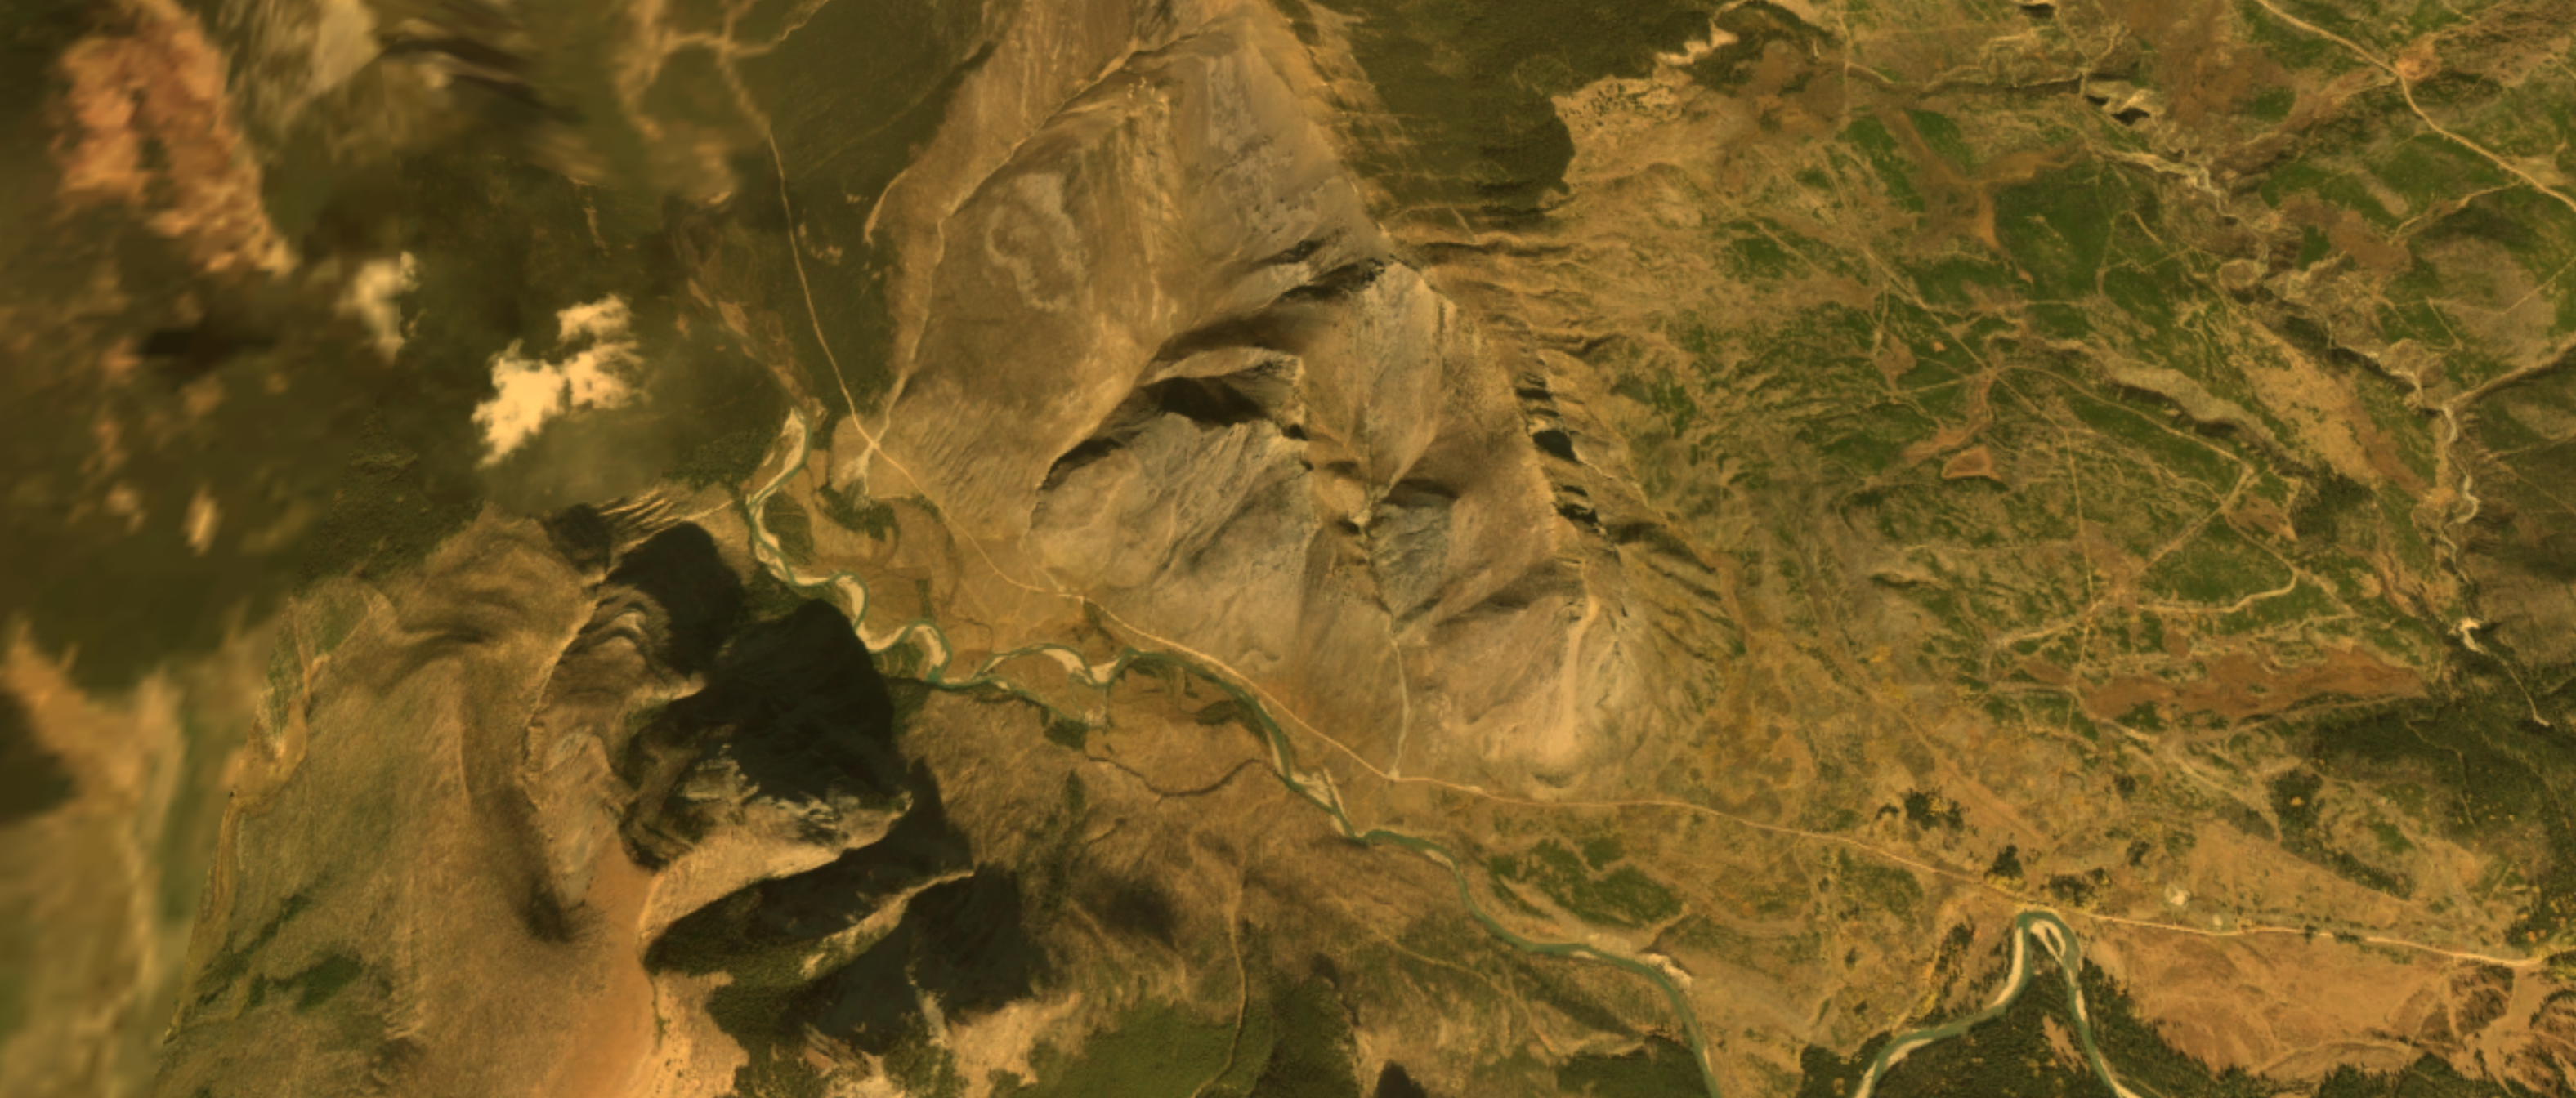
\includegraphics[scale=0.4]{Dogrib3D_1.png}
\caption{\label{fig:Dog1}Dogrib 3D model example: Aerial view}
\end{figure}

A 3D-forest visualization app is generated using the data from the GIS. Then, the user can visit and visualize any point of the virtual terrain (real scale). Examples of this output can be seen in figures \ref{fig:Dog1} to \ref{fig:Dog7}.

\begin{figure}[h!]
\centering
\includegraphics[scale=0.4]{Dogrib3D_2.png}
\caption{\label{fig:Dog2}Dogrib 3D model example: Mountains view}
\end{figure}

\begin{figure}[h!]
\centering
\includegraphics[scale=0.4]{Dogrib3D_3.png}
\caption{\label{fig:Dog3}Dogrib 3D model example: Landscape view}
\end{figure}

As can be seen in the pictures, the visualization app takes into account the position, texture and volume of each component of the terrain in order to generate the 3D-mesh, texturizing it with data collected from satellital services. In addition, light/shadows and weather elements are calculated using online information, giving a ``real and live'' view of the forest state before and after the simulation. 

\newpage

\begin{figure}[h!]
\centering
\includegraphics[scale=0.4]{Dogrib3D_4.png}
\caption{\label{fig:Dog4}Dogrib 3D model example: General view of the instance.}
\end{figure}

\begin{figure}[h!]
\centering
\includegraphics[scale=0.4]{Dogrib3D_5.png}
\caption{\label{fig:Dog5}Dogrib 3D model example: Sunset effect.}
\end{figure}

\newpage

\begin{figure}[h!]
\centering
\includegraphics[scale=0.4]{Dogrib3D_6.png}
\caption{\label{fig:Dog6}Dogrib 3D model example: Transition to night.}
\end{figure}

\begin{figure}[h!]
\centering
\includegraphics[scale=0.4]{Dogrib3D_7.png}
\caption{\label{fig:Dog7}Dogrib 3D model example: Night ambientation.}
\end{figure}

Hence, a completely interactive visualization app is generated by the simulation when using the GIS-based output module.


\newpage

\section{Prometheus: Comparison with deterministic simulator}
Blablabla....

\subsection{Methodology}
Blablabla....

\subsection{Instances}
Blablabla....

\subsection{Results}
Blablabla....

\newpage 

\section{Future/Current Work}
\begin{enumerate}
	\item Gather and test more real life instances with different weather conditions and compare them with existing simulator outputs in order to validate SimName's performance. A series of experiments must be done in order to determine the best value of relevant parameters (like thresholds).
	\item Fire evolution comparison with Prometheus. The current comparisons take into account the last state of the forest (final fire scar), while progressive scars (fire evolution) are not being compared. 	Thus, we would be able to determine if both models present similar fire spread evolutions.
	\item Spotting model: implement a formal spotting model. 
	\item Optimization of SimName functions. A general optimization of the most relevant functions and methods has been performed. Secondary functions will be optimized, taking advantage of parallel/concurrent computing approaches.
	\item An optimized version for HPC (high performance computers) will be finished. It takes advantage of the cluster structure and implements a series of rules for queuing the different jobs among clusters/nodes.
	\item Full integration of the simulator with the GIS module for the 3D-mesh generation. Current beta implementation needs a series of software packages to be installed on the local machine in order to generate the visualization app and three dimensional forest video. Next version will run on an external server, just needing an internet connection.
	\item Formal article (paper): start writting it based on the documents and results we have.
	
\end{enumerate}



\newpage 
\section{Bibliography}
BibTeX.

\bibliographystyle{alpha}
\bibliography{sample}

\newpage



\end{document}
